\chapter{Flexible generative modelling}
\label{ch:flexible-diffusion}

We have now introduced diffusion models in both their unconditional and conditional forms. We have discussed the applications of conditional diffusion models to tasks including text-to-image and text-based image editing. A similarity between these tasks is that we always know in advance what type of data we will condition on at test-time: e.g. for text-to-image we always condition on a text string; for text-based image editing we always condition on a text string and an input image. In other words, the models were trained to work with a single type of conditioning information $\rvy$.

Our thesis is that diffusion models can, in a variety of domains, be made robust to tasks where we do not know what form $\rvy$ will take at test-time. There are many applications where this may be required. For image inpainting, it is desirable to have a single inpainting model that can inpaint any pixels in an image depending on a user's requirements at test time. For video editing (or video generation from keyframes), a user might want to condition on every second frame, every tenth frame, only the first few frames, or so on.

In this chapter we first formalise the idea of a \textit{flexible generative model} which can be used for a large variety of different tasks at test-time without retraining and then we lay out a concrete strategy for implementing and training \textit{flexible diffusion models}.

Ideally we would like to have generative models that need to be trained once and then can be used for \textit{any} conceivable conditioning task at test-time without requiring additional training or data. That is, we would like them to accurately approximate $\pdata(\rvx|\rvy)$ for any possible form of $\rvy$ they are given at test-time and no matter how it is related to $\rvx$. Clearly, though, having a model that can perform \textit{any} conceivable conditioning task is not possible: it wouldn't make sense to train a model on a dataset of images and then expect it to perform text-conditional image generation without ever having seen text data. 
%
To make the idea of flexibility more tractable, we constrain the set of conditioning tasks which we expect to be capable of as follows. We define a flexible generative model to be one that, after being trained with data $\rvx \sim \pdata(\cdot)$, can sample $\rvx$ conditioned on the values of any subset of the components of $\rvx$. For an image generative model, if we treat each pixel as a component, this means being able to condition on any subset of the pixel values. For video tasks, we will consider each frame to be a component and so our flexible video models can be conditioned on any subset of the frame values.

To restate this with notation from \cref{ch:conditional-diffusion}, we will describe what $n_\rvy$ components to condition on with a set of integer indices $\gY = \{ y_1, \ldots, y_{n_\rvy} \}$. We will then define $\rvy = \rvx[\gY] = [ \rvx[y_1], \ldots, \rvx[y_{n_\rvy}] ]$ as a data structure in which the $i$th element is equal to $\rvx[y_i]$. Different $\gY$ correspond to different conditional generation tasks, with the conditional generation task being to generate samples from an approximation of
\begin{equation} \label{eq:flexible-diffusion-target}
    \pdata(\rvx | \rvy, \gY)
\end{equation}
In other words, each conditional generation task is to sample data conditioned on observed components and with knowledge of the index of each observed component. 
%
While we focus on modelling modalities separately, the framework defined here does, in principle, allow flexible generative models to span multiple modalities. If, for example, $\rvx \sim \pdata(\cdot)$ is defined to be an object containing both an image and a text caption, a flexible generative model trained on such data would be capable of any of image captioning, text-to-image generation, or unconditional image and caption generation.

\section{Flexible diffusion objective}

We now present our framework for training diffusion models as flexible generative models, which we call the flexible diffusion framework. Recall that our aim is to approximate the target distribution in \cref{eq:flexible-diffusion-target}. We will denote the approximation of this target from a flexible diffusion model as $p_\theta(\rvx|\rvy,\gY)$. To train this flexible diffusion model we use the objective
\begin{align} \label{eq:flexible-diffusion-loss}
    \mathcal{L}_\text{FDM}(\theta) &= \EX_{u(\sigma)u(\gY)q(\rvx, \rvx_\sigma)\delta(\rvy|\rvx,\gY)} \left[ 
    \frac{\lambda^\rvx(\sigma)}{u(\sigma)} \left\| \predx_\theta(\rvx_\sigma, \rvy, \sigma, \gY) - \rvx \right\|_2^2 \right] \mathrm{d}\sigma.
\end{align}
This flexible diffusion objective is very similar to the conditional diffusion objective in \cref{eq:cond-diffusion-loss}, with the differences being as follows. First, we now have an expectation over $\gY \sim u(\cdot)$. We will call $u(\gY)$ our \textit{training task} distribution and it is up to the developer of a flexible diffusion model to construct it. Second, we now sample $\rvy$ from $\delta(\rvy|\rvx,\gY)$, a Dirac distribution on $\rvy = \rvx[\gY] = [ \rvx[y_1], \ldots, \rvx[y_{n_\rvy}] ]$. One consequence of this manner of sampling $\rvy$ is that it may now have dimensionality that varies between training examples; in fact its dimensionality $n_\rvy$ can now in principle be anywhere between zero and the dimensionality of $\rvx$. Third, we now pass $\gY$ as an extra input into the neural network parameterising $\predx_\theta(\rvx_\sigma, \rvy, \sigma, \gY)$. We will describe how exactly $\gY$ is fed into the neural network for each task in this dissertation as we get to it.

Finally, note that we write the flexible diffusion objective in  \cref{eq:flexible-diffusion-loss} as if we are expecting $\predx_\theta(\rvx_\sigma, \rvy, \sigma, \gY)$ to contain predictions for all components of $\rvx$, even components that are specified in $\gY$ and so observed in $\rvy$. In practice a neural network is not needed to make predictions for these components; we can manually implement functionality that copies these values from the input $\rvy$ into the output $\predx_\theta(\rvx_\sigma, \rvy, \sigma, \gY)$. The squared-error loss for such components will then always be zero. The fact that we include them in the squared-error in \cref{eq:flexible-diffusion-loss} is therefore not important in practice.

\section{Sudoku example}
\begin{figure}[t]
    \centering
    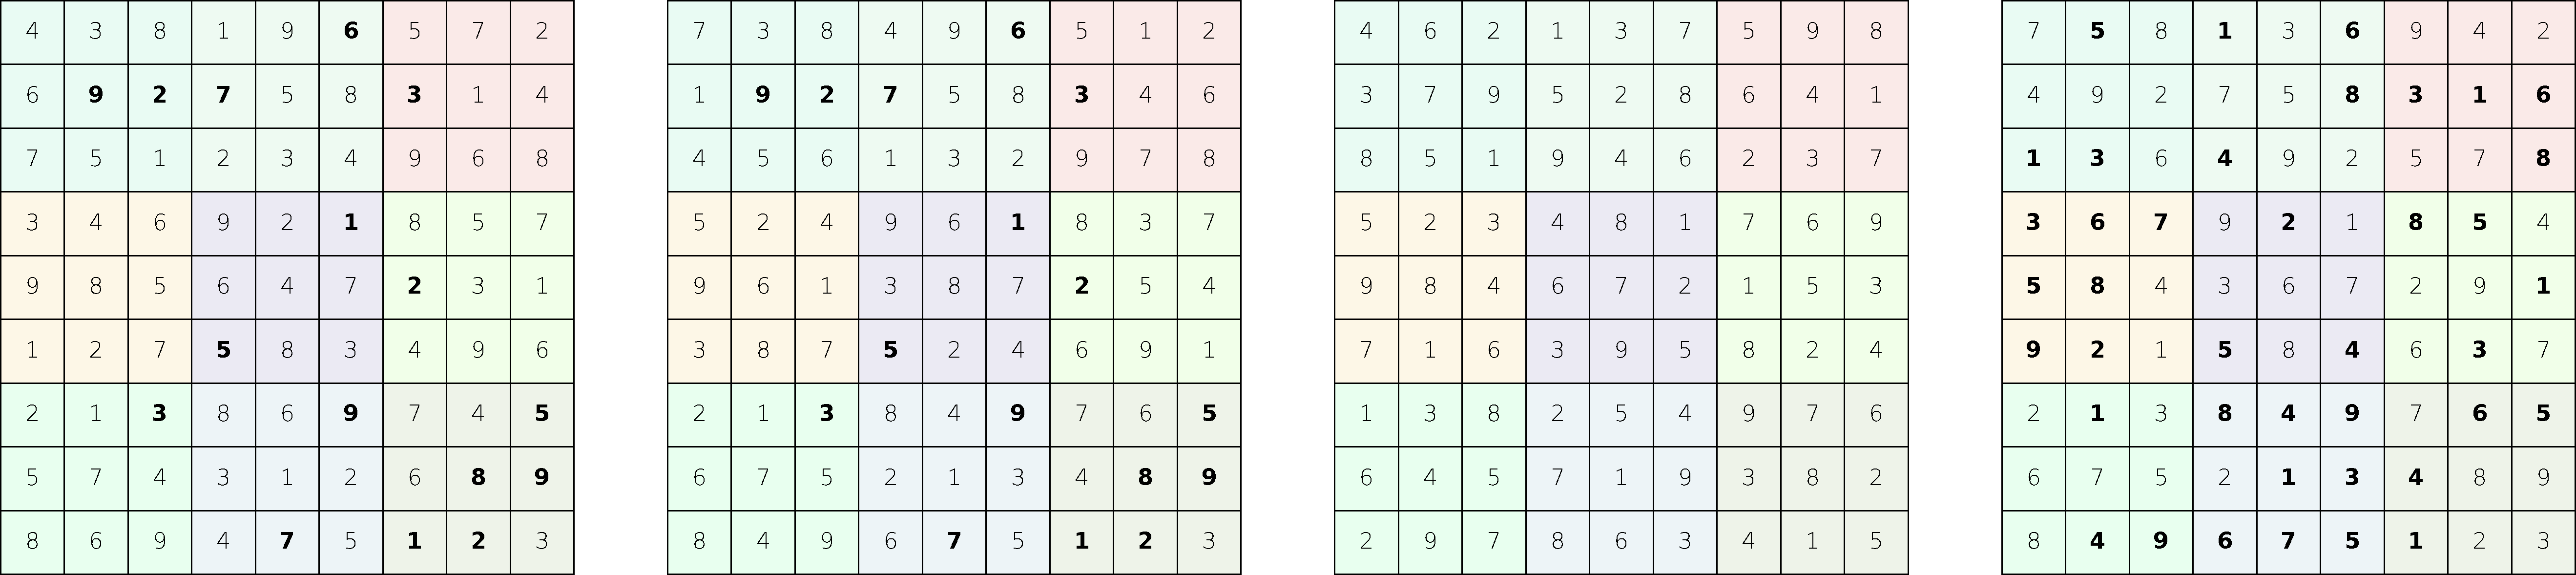
\includegraphics[width=\textwidth]{figs/thesis/sudoku_panel.pdf}
    \caption{Sudoku puzzles solved by a flexible generative model. Observed numbers (i.e. those that form part of $\rvy$) are shown in bold. The observed numbers are the same for the leftmost two Sudokus but multiple solutions exist, and we show that the generative model is able to find two different solutions. In the third Sudoku from the left, no numbers were observed. This corresponds to the task with $\gY = \{\}$. The training task distribution $u(\gY)$ covered such tasks and so this flexible generative model is capable of unconditional generation as shown. }
    \label{fig:sudoku-panel}
\end{figure}
We end this section with an intuitive example of a task where flexible conditioning is required: solving Sudoku puzzles~\citep{weilbach2023graphically}. A Sudoku is a $n^2 \times n^2$ grid of integers, each of which takes a value in $\{1,\ldots,n^2\}$. Most commonly, $n$ is set to three so the grid has size $9 \times 9$. There are three types of constraint required for a Sudoku to be valid: no value can appear more than once within the same row of the grid; no value can appear more than once within the same column; and no value can appear more than once within any of the $n^2$ $n \times n$ sub-grids that make up the grid. Sudoku puzzles are puzzles in which the player is given a Sudoku with values missing. The player is then required to fill in the missing values. Most puzzles are constructed to have a single solution, but if the values in sufficiently few cells are given then multiple solutions can be possible. We can frame solving Sudokus as a conditional generative modelling problem if we have a data distribution $\pdata(\rvx)$ that places probability mass over all complete and valid Sudoku grids.\footnote{Fortunately this distribution is efficient to sample from. We follow the procedure from \url{https://turtletoy.net/turtle/5098380d82}.} The set of observed indices $\gY$ denotes which cells the user is given values for, and the user must infer the values for all cells not in $\gY$. The cells whose values are given as clues vary between different Sudoku puzzles, and so training a conditional generative model that can solve any given Sudoku puzzle means training a flexible generative model. 

We trained a flexible diffusion model with a very simple training task distribution that uniformly samples how many cells to observe the values of from between zero and $n^4-1$ (the number of cells minus one) and then uniformly samples this many cell indices to construct $\gY$. We process the input to the neural network by replacing elements of $\rvx_\sigma$ corresponding to observed values with those observed values. The network then performs a linear projection of each resulting value and adds a learned embedding to elements with observed values. This forms the input to a transformer-based architecture~\citep{vaswani2017attention}. We refer to \citet{weilbach2023graphically} for further details of the architecture and training procedure. \Cref{fig:sudoku-panel} shows a variety of Sudoku puzzles solved by our flexible diffusion model.

\section{Outline of the remaining chapters}
In the chapters that follow we will expand on the flexible generative modelling framework in several ways. First, in \cref{ch:fdm}, we will define a flexible diffusion model that is capable of ``marginalising out'' components in the original data that we do not wish to sample or condition on. To do so we will modify \cref{eq:flexible-diffusion-target} to additionally condition on $\gX$, the indices of components we wish to generate and then sample the values of only those $|\gX|$ elements. This will let us scale the flexible generative modelling framework to large and complex data in the form of long videos. In \cref{ch:tddm} we will explore how to build flexible generative models for the case where the data has varying dimensionality and $\pdata(\rvx | \rvy, \gY)$ is a trans-dimensional distribution from which different samples can have different dimensionality. In this case, conditioning on $\gY$ also implies conditioning on $\rvx$ having at least as many components as suggested by the largest index in $\gY$. In \cref{ch:cigcvae} we will explore how to build a flexible generative model for the image domain based on the variational auto-encoder framework. We end by discuss our final conclusions and outlook in \cref{ch:conclusion}.
